\documentclass[11pt,a4paper]{article}
\usepackage[margin=0.85in]{geometry}
\usepackage[T1]{fontenc}
\usepackage{lmodern}
\usepackage{amsmath,amssymb,mathtools}
\usepackage{graphicx,booktabs,array,enumitem}
\usepackage[dvipsnames]{xcolor}
\usepackage{microtype}
\usepackage{caption}
\usepackage{listings}
\usepackage{hyperref}
\hypersetup{colorlinks=true,linkcolor=MidnightBlue,urlcolor=MidnightBlue,
  pdfauthor={},pdfsubject={Reinforcement learning worked solutions}}
\setlength{\parindent}{0pt}
\setlength{\parskip}{6pt}
\setlist{nosep,leftmargin=*}
\setlength{\emergencystretch}{2em}
\captionsetup{font=small,labelfont=bf}
\lstset{basicstyle=\ttfamily\small,breaklines=true,
  columns=fullflexible,keepspaces=true,showstringspaces=false,
  commentstyle=\color{gray},keywordstyle=\color{MidnightBlue},
  aboveskip=6pt,belowskip=6pt}
\newcommand{\E}{\mathbb{E}}
\newcommand{\R}{\mathbb{R}}
\newcommand{\norm}[1]{\left\lVert #1\right\rVert}
\newcommand{\sg}{\operatorname{stopgrad}}
\DeclareMathOperator*{\argmax}{arg\,max}
\DeclareMathOperator*{\argmin}{arg\,min}
\newcommand{\studytitle}[1]{%
  \hypersetup{pdftitle={#1 - Worked Solutions}}%
  {\small\color{MidnightBlue} BASICRL\quad /\quad WORKED SOLUTIONS}\par
  \vspace{5pt}{\LARGE\bfseries #1}\par\vspace{5pt}}
\newcommand{\historical}{\textbf{Experiment status.} The following numbers and
  curves are retained from earlier runs, not from a rerun of the revised
  reference code. They are examples for interpretation, not performance guarantees.\par}

\begin{document}
\studytitle{Actor-Critic and Policy Improvement}

\section{Approximate policy improvement}
Consider a discounted MDP with bounded rewards and $0<\gamma<1$. Suppose
$\norm{V^\pi-\widehat V}_\infty\leq\epsilon$. Define the Bellman operators
\[
 (T_\rho v)(s)=r_\rho(s)+\gamma(P_\rho v)(s),\qquad
 (Tv)(s)=\max_a\{r(s,a)+\gamma(P_av)(s)\}.
\]
A greedy policy $\widehat\pi$ satisfies $T_{\widehat\pi}\widehat V=T\widehat V$,
which is pointwise at least $T_\pi\widehat V$. This also covers a stochastic
reference policy because a maximum dominates any mixture of actions.

\subsection{The one-step error}
Write $e=V^\pi-\widehat V$ and $\Delta=V^\pi-V^{\widehat\pi}$. By the two
Bellman equations and the greedy inequality,
\begin{align*}
 \Delta
 &=T_\pi V^\pi-T_{\widehat\pi}V^{\widehat\pi}\\
 &\leq\gamma P_\pi e
           +\gamma P_{\widehat\pi}(\widehat V-V^{\widehat\pi})\\
 &=\gamma P_\pi e-\gamma P_{\widehat\pi}e
                                +\gamma P_{\widehat\pi}\Delta\\
 &\leq2\gamma\epsilon\,\mathbf1+\gamma P_{\widehat\pi}\Delta.
\end{align*}
The last line uses $|e(s)|\leq\epsilon$ and the fact that each transition
row sums to one. The factor 2 accounts for the two action-dependent
continuations compared using the approximate value.

\subsection{Closing the recurrence}
Iterate the inequality $n$ times:
\[
 \Delta\leq2\gamma\epsilon\sum_{k=0}^{n-1}\gamma^k\mathbf1
               +\gamma^n P_{\widehat\pi}^n\Delta.
\]
Bounded rewards imply bounded values, so the last term tends uniformly to 0.
Taking $n\to\infty$ yields
\[
 \boxed{V^\pi(s)-V^{\widehat\pi}(s)
          \leq\frac{2\gamma\epsilon}{1-\gamma}\quad\text{for every }s.}
\]
This is a \emph{one-sided} guarantee relative to the reference policy. It
does not bound $|V^\pi-V^{\widehat\pi}|$: the greedy policy can be much
better than the reference. It is not an optimality-gap bound unless the
reference itself is optimal.

\newpage
\section{Why the horizon matters}
An approximate greedy choice can lose up to $2\gamma\epsilon$ in a one-step
comparison. Future choices can incur similar losses, and the discounted
sum of their weights is $1+\gamma+\gamma^2+\cdots=1/(1-\gamma)$. This
explains the effective-horizon factor. The derivation accumulates a
discounted sequence of losses; it does not assert exponential growth in time.

When $\epsilon=0$, the bound reduces to ordinary policy improvement:
$V^{\widehat\pi}\geq V^\pi$. As $\gamma\to1$, long-range consequences
make the same approximation accuracy provide a weaker infinite-horizon guarantee.

\section{A precise finite-horizon version}
Let the decision times be $t=0,\ldots,H-1$, with common zero terminal value
$V_H^\pi=V_H^{\widehat\pi}=\widehat V_H=0$. Assume, at \emph{each time},
\[
 \norm{V_t^\pi-\widehat V_t}_\infty\leq\epsilon_t.
\]
Choose the time-dependent policy
\[
 \widehat\pi_t(s)\in\argmax_a
       \{r_t(s,a)+\gamma P_{t,a}\widehat V_{t+1}(s)\}.
\]
Repeating the one-step proof gives
\[
 \Delta_t\leq2\gamma\epsilon_{t+1}\mathbf1
                 +\gamma P_{t,\widehat\pi_t}\Delta_{t+1},\qquad\Delta_H=0.
\]
Therefore
\[
 \boxed{\Delta_0(s)\leq2\sum_{t=0}^{H-1}\gamma^{t+1}\epsilon_{t+1}.}
\]
For $\epsilon_t\leq\epsilon$ at nonterminal times and $\epsilon_H=0$,
\[
 \Delta_0(s)\leq
 \begin{cases}
 2\gamma\epsilon\dfrac{1-\gamma^{H-1}}{1-\gamma},&0<\gamma<1,\\[5pt]
 2(H-1)\epsilon,&\gamma=1.
 \end{cases}
\]
With only one action remaining ($H=1$), the terminal continuation is exact,
so this bound is zero. The looser $2H\epsilon$ order statement is often
useful, but the time indexing and terminal condition are needed to justify it.
A single stationary estimate of an infinite-horizon value does not automatically
satisfy these finite-horizon assumptions.

\newpage
\section{Actor and critic objectives}
\subsection{Monte Carlo advantage actor-critic}
For the notebook's episodic discounted objective, let
$G_t=\sum_{u=t}^{T-1}\gamma^{u-t}r_u$ and $A_t=G_t-V_\phi(s_t)$. Use
\[
 L_{\rm actor}=-\sum_t\gamma^t\log\pi_\theta(a_t\mid s_t)\sg(A_t),\qquad
 L_{\rm value}=\frac1T\sum_t(V_\phi(s_t)-G_t)^2.
\]
This implementation uses full sampled returns and a learned baseline. It
is not the one-step temporal-difference version of A2C. Keep both values and
returns shaped $(T,)$ to avoid accidentally broadcasting into $(T,T)$.
Detaching the advantage prevents the actor objective from updating the critic.

\subsection{DDPG}
Sample transitions $(s,a,r,s',d)$ from replay, where $d$ is the true terminal
mask under the chosen task definition. With target networks denoted by bars,
\[
 y=r+\gamma(1-d)Q_{\bar\phi}(s',\mu_{\bar\theta}(s')),
 \quad L_Q=\E[(Q_\phi(s,a)-\sg(y))^2],
 \quad L_\mu=-\E[Q_\phi(s,\mu_\theta(s))].
\]
Exploration adds noise to the behavior action; it is omitted for deterministic
evaluation. Slowly update targets with
$\bar\phi\leftarrow(1-\tau)\bar\phi+\tau\phi$ and likewise for the actor.

\subsection{SAC and the squashed Gaussian}
For twin critics and entropy temperature $\alpha>0$,
\begin{align*}
 y&=r+\gamma(1-d)
  \left[\min_{j=1,2}Q_{\bar\phi_j}(s',a')-\alpha\log\pi_\theta(a'\mid s')\right],\\
 L_{\pi}&=\E[\alpha\log\pi_\theta(a\mid s)-\min_jQ_{\phi_j}(s,a)],
 \qquad a'\sim\pi_\theta(\cdot\mid s').
\end{align*}
Use reparameterized sampling $u=\mu+\sigma\odot\xi$, $\xi\sim N(0,I)$,
and $a=b+c\odot\tanh u$. For positive action scales $c_i$,
\[
 \log\pi(a\mid s)=\sum_i\left[
    \log N(u_i;\mu_i,\sigma_i^2)-\log c_i-\log(1-\tanh^2u_i)\right].
\]
The Jacobian correction is essential. Store action scales as registered
buffers so they follow the module to its device. Reset an ordinary environment
after termination or truncation. For an external time-limit cutoff of a
continuing task, reset the rollout but retain bootstrapping; true terminal
transitions suppress the bootstrap. A finite-horizon task must include its
remaining-time convention in the state and terminal definition.

\newpage
\section{Retained experiments and interpretation}
\historical
The saved evaluation outputs include actor-critic returns around $1.74$,
DDPG around $1.64$, and SAC around $1.64$--$1.66$. These values use the
fixed-goal progress reward; they are not directly comparable with the sparse
reward in the imitation-learning topic. They also lack repeated-seed
confidence intervals, so they do not establish an algorithm ranking.

\begin{figure}[h!]
\centering
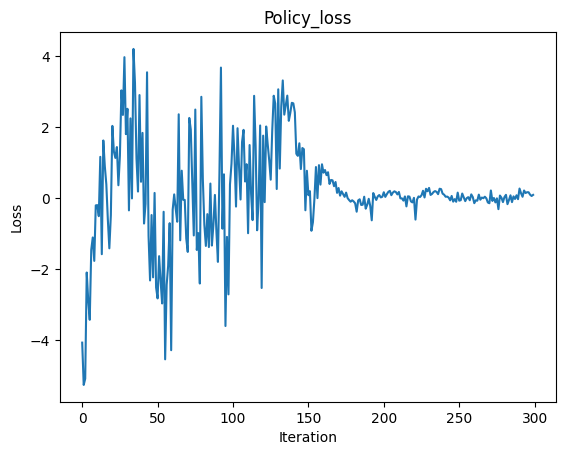
\includegraphics[width=0.47\linewidth]{figures/advantage-actor-loss.png}\hfill
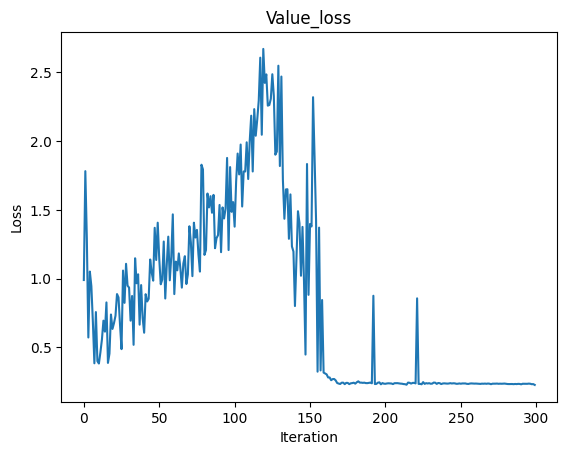
\includegraphics[width=0.47\linewidth]{figures/advantage-critic-loss.png}
\caption{Historical actor and critic losses for the advantage-baseline method.}
\end{figure}
\begin{figure}[h!]
\centering
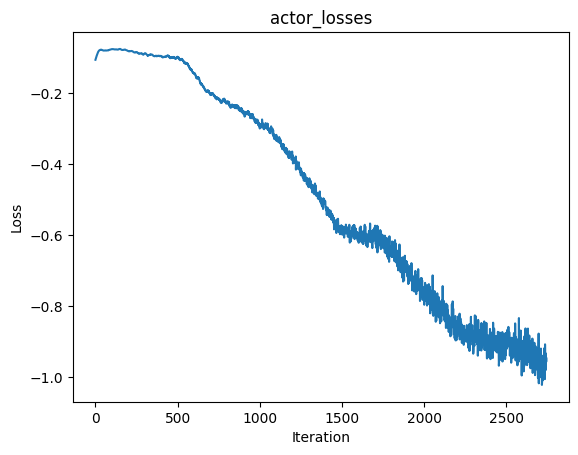
\includegraphics[width=0.47\linewidth]{figures/ddpg-actor-loss.png}\hfill
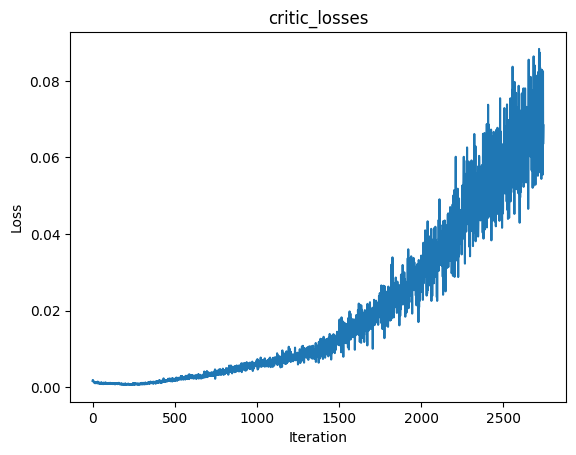
\includegraphics[width=0.47\linewidth]{figures/ddpg-critic-loss.png}
\caption{Historical DDPG losses. A growing critic loss can accompany changing
targets or state distributions; interpret it alongside evaluation returns.}
\end{figure}
The revised code addresses episode resets, replay-buffer interfaces, terminal
masks, batch sizes, device buffers, and actor-loss shape and discount conventions.
The saved curves predate those corrections. Re-run the notebooks before
claiming any performance for the revised implementation.

\textbf{Solution scope.} The one-sided infinite-horizon bound and the
time-indexed finite-horizon bound follow under their explicit approximation
assumptions. The practical losses specify the corresponding algorithms;
the retained curves are observational records rather than convergence proofs.
\end{document}
